\documentclass{article}
\usepackage[utf8]{inputenc}
\usepackage{graphicx}

\title{B-Spline Curvature Constraint Approaches}
\author{davidc}
\date{July 2022}

\begin{document}

\maketitle

\section{Introduction}

This paper covers various approaches to constrain the curvatures of a B-spline with varying degrees of speed, accuracy, and boundedness. The objective is to find the maximum curvature of a B-spline for each knot-point interval.

\section{Preliminaries}

The curvature at specific point is defined by the circle that best approximates the shape of the curve at that point. It is formally defined by the inverse radius of the circle. See figure \ref{Fig:Curvature}. 

\begin{figure}[h]
\begin{center}
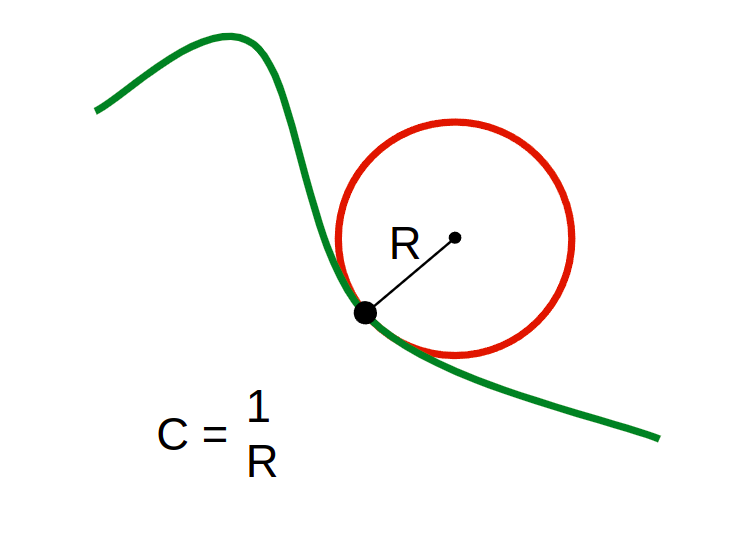
\includegraphics[scale=.23]{Curvature.png}
\end{center}
\caption{Curvature defined by the oscillating circle}
\label{Fig:Curvature}
\end{figure}

The curvature of a B-spline \(b(t)\) with first and second derivatives \(b(t)'\) and \(b(t)''\) is defined as follows.

\begin{equation}
    C(t) = \frac{||b_{(t)}' \times b_{(t)}''||}{||b_{(t)}'||^3}
\end{equation}

Using the rules for the derivative of a cross product and the derivative of a norm, we can show the derivative of the curvature. We also use the third derivative of the spline \(b(t)'''\). See appendix for derivative rules.

\begin{equation}
    C(t)' = \frac{(b_{(t)}' \times b_{(t)}'') \cdot (b_{(t)}' \times b_{(t)}''')}{||b_{(t)}' \times b_{(t)}''||\;||b_{(t)}'||^3} - \frac{3(b_{(t)}' \cdot b_{(t)}'') || b_{(t)}' \times b_{(t)}''||}{||b_{(t)}'||^5}
\end{equation}


We can also define the curvature with the portion of the second derivative that is perpendicular to the first derivative.

\begin{figure}[h]
\begin{center}
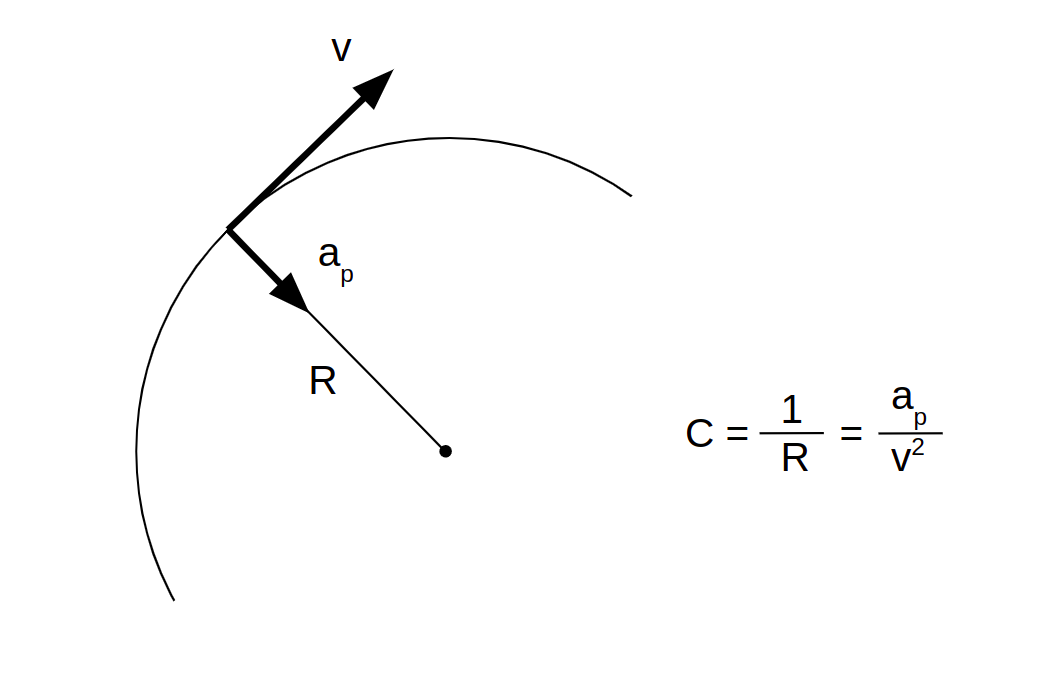
\includegraphics[scale=.23]{Centripetal_Acceleration.png}
\end{center}
\caption{Centripetal Acceleration Equation}
\label{Fig:Centripetal_Acceleration}
\end{figure}

\begin{equation}
    C(t) = \frac{||b_{(t)}_p''||}{||b_{(t)}'||^2}
\end{equation}

where the perpendicular portion of the second derivative is equal to the following.

\begin{equation}
    b(t)_p'' = b_{(t)}'' -  \Bigl(b_{(t)}' \cdot b_{(t)}''\Bigl) \frac{b_{(t)}'}{||b_{(t)}'||^2}
\end{equation}

This relation comes from the equation for centripetal acceleration. See Figure (\ref{Fig:Centripetal_Acceleration}).


\section{Motivation}




\section{SQP Over the Curvature Equation}

\section{Appendix}

\begin{equation}
    \frac{d}{dt} ||a|| = \frac{a \cdot \frac{da}{dt}}{||a||}
\end{equation}

\begin{equation}
    \frac{d}{dt} (a \times b) = \frac{da}{dt} \times b +  a \times \frac{db}{dt}
\end{equation}

\begin{equation}
    
\end{equation}

\end{document}
